\documentclass[8pt]{beamer}

\usepackage[utf8]{inputenc}
\usepackage{default}
\usepackage{hyperref}
\usetheme{Copenhagen}

\title{Deep Learning}
\subtitle{Learning High-degree Non-linear Models: \\
Enabling factors, tips and tricks}
\author{Tero Keski-Valkama}
\institute{Cybercom}
\date{2016-08-24}
\logo{\includegraphics[height=1.5cm]{cybercom-blue.png}}

\begin{document}

\frame{\titlepage}
 
\begin{frame}
\frametitle{A quick recap}
\begin{itemize}
 \item Deep learning refers to deep neural networks. It took about 10 years for neural network technology to
       surpass the issues they stalled with in the 1990s. In 00s, if an academic paper mentioned neural networks, it was less likely to be published than if not.
 \item 1990s networks were shallow, and hence relatively useless: It requires a bunch of non-trivial tricks to make deeper networks possible.
       This presentation will present the most important of these tricks.
 \item Neural networks are just complex non-linear models with lots of parameters. They are formed by layers of neurons, successive operations
       with an a linear combination of inputs from the previous layer and an activation function.
 \item In general, you always need a training set, a test set and a validation set. Typically you would divide your data into three parts,
       train the system with the training set, test if the system overfits with the test set, and finally for the final system you can validate
       that your metaparameters didn't just learn the test set using the validation set.
 \item Underfitting = high bias, overfitting = high variance
\end{itemize}

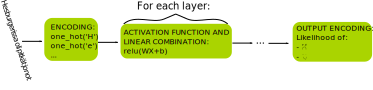
\includegraphics[width=0.9\textwidth]{./sentiment_analysis.png}

\end{frame}

\begin{frame}
\frametitle{Training Neural Networks 1/2}
\begin{itemize}
 \item Networks can be trained in a supervised fashion, with target outputs(labels), using backpropagation of error.
       The output error is known, and it is propagated backwards, layer by layer, estimating an error for each weight parameter.
       The weights are then updated using this error multiplied by the learning factor ($ << 1 $). Lots of learning steps makes
       the network learn the target function ($ input \rightarrow target\_output $)
 \item Non-linearities (activation functions) between the layers make the model interesting, compared to other statistical models.
 \item When the layers are getting smaller than the previous layer, the information is being compressed (or filtered), and the layer
 activations represent a higher abstraction level, a higher semantic level information about the signal.
\end{itemize}
\end{frame}

\begin{frame}
\frametitle{Training Neural Networks 2/2}
\begin{itemize}
 \item Unsupervised learning (no target output) can be done using backpropagation and autoassociativity ($ input \rightarrow input $),
 (or prediction: $ delayed\_input \rightarrow input $), or using Deep Belief Nets and Contrastive Divergence
 \footnote{\href{http://deeplearning.cs.cmu.edu/notes/yuxiong\_CD.pdf}{http://deeplearning.cs.cmu.edu/notes/yuxiong\_CD.pdf}}
 (minimizes the energy
 for generating real data-related distributions while maximizing the energy for "confabulations") for pairs of subsequent layers one by one.
 \item Metaoptimizing the learning hyperparameters and neural network structure should always be performed.
 \item A good platform to use for neural network experimentation is Google's TensorFlow, based on Python.
\end{itemize}

\begin{tabular}{| c | c |}
\hline
Supervised & Unsupervised \\
Backpropagation & Contrastive Divergence \\
Non-energy-based Methods & Energy-based Methods \\
\hline
 
\end{tabular} 

\end{frame}

\begin{frame}
\frametitle{Tips \& Tricks}
 \begin{block}{Problems}
  \begin{itemize}
   \item Overlearning
   \item Getting stuck in local minima
   \item Exploding/diminishing gradients
  \end{itemize}
 \end{block}

 \begin{block}{Solutions}
  \begin{enumerate}
   \item Weight-sharing – less parameters
   \item Unsupervised pre-training – lots of data
   \item Near-linear activation functions
   \item Drop-out
   \item Gradient clipping
   \item Metaoptimization
   \item Bonus: Reservoir computing 
  \end{enumerate}
 \end{block}

\end{frame}

\begin{frame}
\frametitle{Regularization and Weight Sharing}
 \begin{itemize}
  \item Reducing the number of parameters or degrees of freedom of the model is regularization. Regularization prevents overfitting.
  \item In Convolutional Neural Networks, the weights are identical for each window, and window outputs are max-pooled (sub-sampling) to the next layer.
        This exploits the translational symmetry of the domain, and is often used for images.
  \item Regularization can also be done by introducing a loss term for weights, L2 norm is often used.
  \item As always in multiobjective optimization, the factors and slopes of the loss function components are important.
 \end{itemize}
 \begin{displaymath}
  RegularizedLoss = Loss + \alpha \cdot SquaredWeights^\beta
 \end{displaymath}
 \includegraphics[width=0.9\textwidth]{./Typical_cnn.png}
 \footnote{Image from: Aphex34, Wikipedia}
\end{frame}



\end{document}




